\documentclass{beamer}
\usepackage{lsfolien}
\usepackage[main=english,ngerman]{babel}
\usepackage[utf8]{inputenc}

\myfootline{System Modelling and Semantic Web -- Winter Term 2021}{Hans-Gert
  Gräbe}

\newcommand{\ueberschrift}[1]{\begin{center}\bf #1\end{center}}

\title{Modelling Sustainable Systems\\ and Semantic Web\\[6pt]
  Systems, Sustainability, Development
  \vskip1em}

\subtitle{Lecture in the Module 10-202-2309\\ for Master Computer Science}

\author{Prof. Dr. Hans-Gert Gräbe\\
\url{http://www.informatik.uni-leipzig.de/~graebe}}

\date{October 2021}
\begin{document}

{\setbeamertemplate{footline}{}
\begin{frame}
  \titlepage
\end{frame}}

\begin{frame}{Sustainability and Challenges}\LARGE

  What do you understand by \textbf{sustainability}

  and what are the \textbf{challenges facing humanity} today? 

\end{frame}

\begin{frame}{Notes on Possible Responses}

Climate change
\begin{itemize}
\item Importance of climate stress for the development of humankind.
\end{itemize}

Hans Carl von Carlowitz and his definition of sustainability.
\begin{itemize}
\item What problems faced the royal Polish and electoral Saxon chamberlain,
  mountain councillor and chief miner of the Ore Mountains
  (königlich-polnischer und kurfürstlich-sächsischer Kammer- und Bergrat sowie
  Oberberghauptmann des Erzgebirges)?
\end{itemize}
\end{frame}

\begin{frame}{Notes on Possible Responses}
17 Sustainable Development Goals (SDG) 
\begin{itemize}
\item Important step of operationalisation in the context of a significant
  political process.
\item It takes up the categorical imperative of Marx and the socialist
  movement to "Overthrow all conditions in which man is a degraded, a
  subjugated, an abandoned, a contemptible being."\medskip

  (Alle Verhältnisse umwerfen, in denen der Mensch ein erniedrigtes, ein
  geknechtetes, ein verlassenes, ein verächtliches Wesen ist.)
\end{itemize}
\end{frame}

\begin{frame}{Notes on Possible Responses}
  However, Marx' original states
  \begin{quote}\rm
    The critique of religion ends with the doctrine that \emph{man is the
      highest being for man}, that is, with the \emph{categorical imperative
      to overthrow all relations} in which man is a degraded, a subjugated, an
    abandoned, a contemptible being (MEW 1, 385).\medskip

    Die Kritik der Religion endet mit der Lehre, dass \emph{der Mensch das
      höchste Wesen für den Menschen} sei, also mit dem \emph{kategorischen
      Imperativ, alle Verhältnisse umzuwerfen}, in denen der Mensch ein
    erniedrigtes, ein geknechtetes, ein verlassenes, ein verächtliches Wesen
    ist.
  \end{quote}
  This imperative is motivated by the relationship of man to man, thus it
  moves within a \emph{specific system}, the social system, and does not
  thematise the relationship to "nature" (it is an early work by Marx).
\end{frame}

\begin{frame}{Digression: Analysing the Challenges using TRIZ}

  \ueberschrift{Peak Oil -- Still an Issue?}

  \begin{center}
    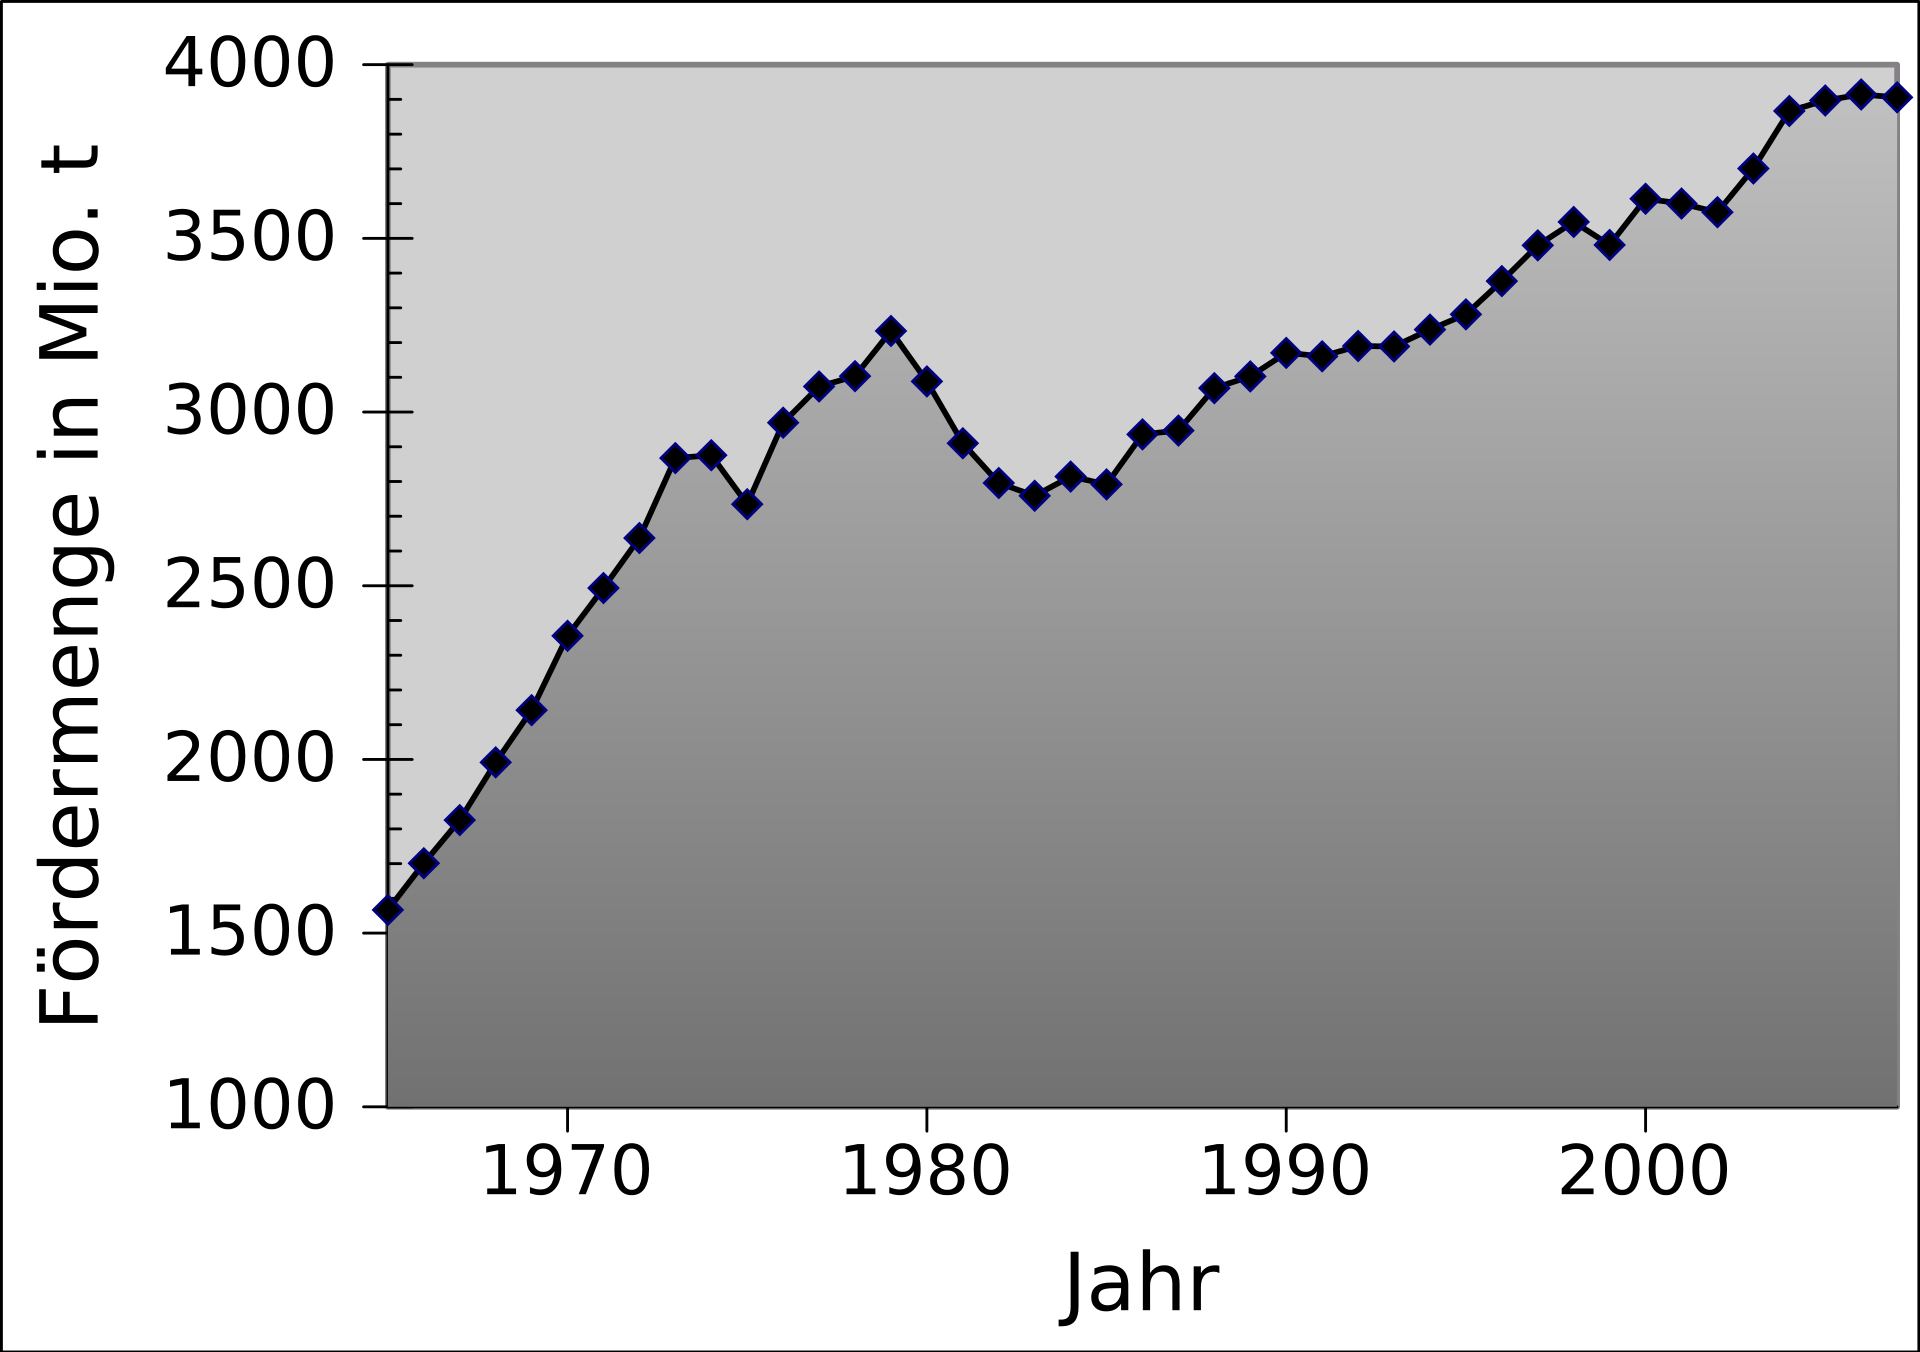
\includegraphics[width=.6\textwidth]{Bilder/9B7Cna.png}
  
    World oil production 1967 -- 2007. Source: Wikipedia
  \end{center}
\end{frame}

\begin{frame}{Peak Oil -- Still an Issue?}

  \begin{center}
    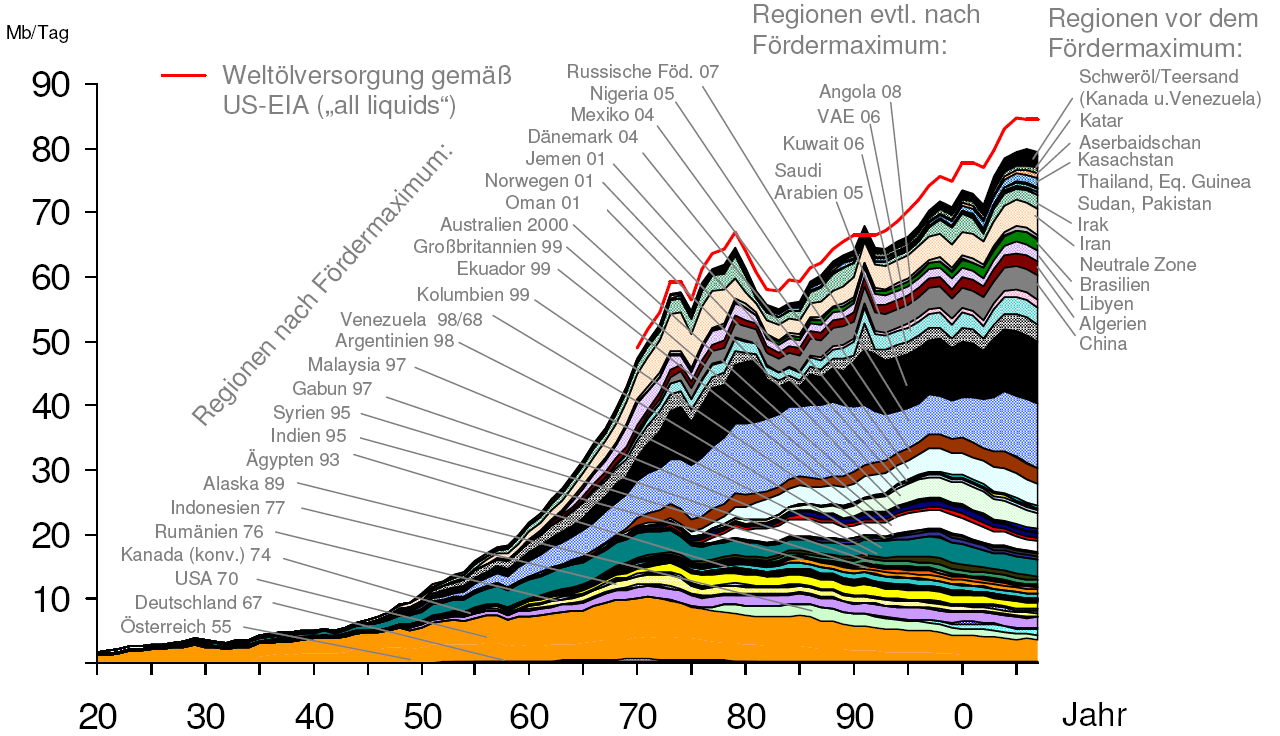
\includegraphics[width=.95\textwidth]{Bilder/ZNEj4U.png}
  
    World oil production over the last 100 years. Source: Wikipedia
  \end{center}
\end{frame}

\begin{frame}{Analysing the Challenges using TRIZ}
  TRIZ rule -- model and go to extreme parameter values.

  Here: Fitting of a Gaussian curve $f(t)=e^{\frac{-x^2}{1764}}$, such that 20
  years before the maximum, 80\% of the maximum is reached.
  \begin{center}
    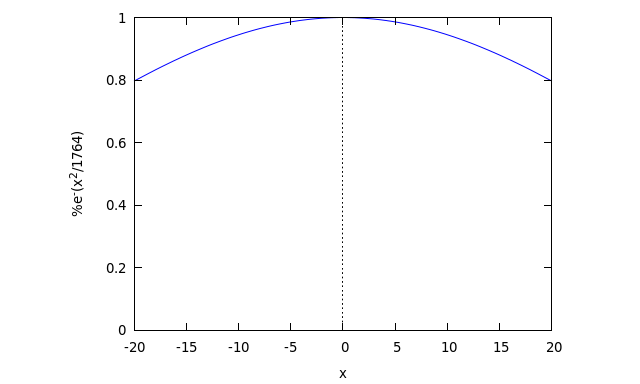
\includegraphics[width=.8\textwidth]{Bilder/aA9bD9.png}
  \end{center}
\end{frame}

\begin{frame}{Analysing the Challenges using TRIZ}
  TRIZ rule -- model and go to extreme parameter values.
  \begin{center}
    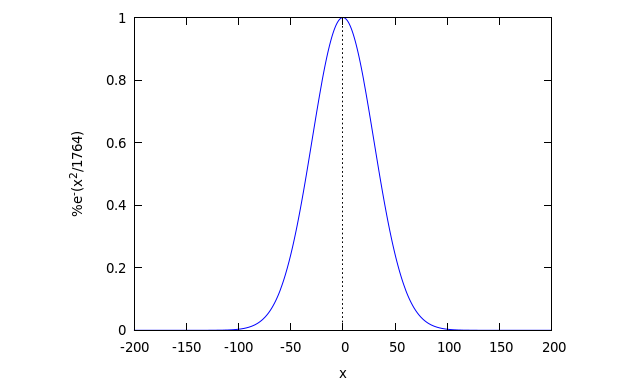
\includegraphics[width=.45\textwidth]{Bilder/RMZ1it.png}\hfill
    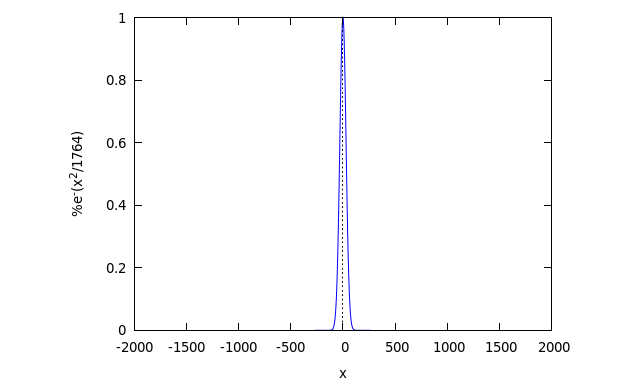
\includegraphics[width=.45\textwidth]{Bilder/mP650q.png}
  \end{center}
\end{frame}

\begin{frame}{Analysing the Challenges using TRIZ}
  The industry of the 20th century has brought us prosperity and wealth.  but
  also
\begin{itemize}
\item Pollution, the hole in the ozone layer,
\item Problems of extensive agriculture,
\item Progressive desertification (Aral Sea),
\item Insect extinction, global warming,
\item Overexploitation of the rainforest ...
\end{itemize}

\textbf{Fundamental insight:} Economic activity based on fossil resources
cannot be sustainable in the long term.

\textbf{Problem:} How can this insight be implemented into the negotiating and
decision-making structures of the bourgeois world society?
\end{frame}

\begin{frame}{Analysing the Challenges using TRIZ}
  \begin{itemize}
  \item It is not (only) about "climate change", "species extinction" etc.,
    but about the dynamics of the "fossil age" and the regenerative capacity
    of the nature we are "exploiting".
  \item Economies based on fossil resources cannot be sustainable in the
    long term.  
  \end{itemize}
\end{frame}

\begin{frame}{Analysing the Challenges using TRIZ}
  
\textbf{Problem:} The mode of production based on fossil resources is not
sustainable.

It is useful and harmful at the same time:
\begin{itemize}
\item Useful (short term)
  \begin{itemize}
  \item Makes life easier
  \item Increases power of action
  \end{itemize}
\item Harmful (long term)
  \begin{itemize}
  \item Undermines the conditions of existence of humanity.
  \end{itemize}
\end{itemize}
\end{frame}

\begin{frame}{Analysing the Challenge using TRIZ}
We want to analyse the Challenge according to
\begin{itemize}
  \item Operational time
  \item Requirements (Ideal Final Result)
  \item Historical Optimism
  \item System Level
  \item Central Instruments and
  \item Contradiction Approach
\end{itemize}
\end{frame}

\begin{frame}{Analysing the Challenge using TRIZ}
  \textbf{Operative time} -2000 .. +2000
  \begin{itemize}
  \item \textbf{Ideal final result:} Complete transformation of the mode of
    production to cycles that use solely the dissipative material and energy
    throughput that is permanently supplied by sun.
  \item \textbf{Historical optimism:} For over 1000 years we have managed more
    or less well to transform the Earth's natural landscape into a cultural
    landscape.
  \item \textbf{System level:} Work as permanent confrontation with the global
    living conditions of humankind.
  \item \textbf{Central instruments:} Technology and science
  \item \textbf{Contradiction approach:} Technology and science in the current
    version are charged with the same contradictions as the mode of production
    -- useful in the short term, harmful in the long term.
  \end{itemize}
\end{frame}

\begin{frame}{Analysing the Challenge using TRIZ}
  \textbf{Operative time} -200 .. +200\small
  \begin{itemize}
  \item \textbf{Ideal final result:} Technology and science must be
    transformed in such a way that primary cost-benefit thinking (at the level
    of the economic system) is replaced by closed-loop thinking as an
    essential element of the transformation of the mode of production
    (at the level of the supersystem).
  \item \textbf{Historical optimism:} In the last 200 years, we have always
    managed again and again to adapt bourgeois society to new conditions of
    technology and science.
  \item \textbf{System level:} Development of technology and science as
    essential instruments in shaping our global living conditions.
    (Supersystem as component!)
  \item \textbf{Central instruments:} Negotiation and decision-making
    structures of bourgeois society.
  \item \textbf{Contradiction approach:} Inability to take into account the
    long-term interests of humanity in the given power structures.
  \end{itemize}
\end{frame}

\begin{frame}{Analysing the Challenge using TRIZ}
  \textbf{Operative time} -20 .. +20\small
  \begin{itemize}
  \item \textbf{Ideal final result:} The structures of negotiation and
    decision-making of the bourgeois society have to be transformed in such a
    way that long-term human interests are better taken into account
    (super-super-system) and technology and science are oriented differently
    (super-system).
  \item \textbf{Historical optimism:} In the long term, this is a central part
    of the negotiating structures of bourgeois society (Starting from
    "liberty, equality, fraternity" of the French Revolution in 1789 to the UN
    "Declaration of Human Rights" in 1947 and Article 1 of the German
    Constitution (Grundgesetz)).
  \item \textbf{System level:} Negotiation and decision-making structures of
    the civil bourgeois society.
  \end{itemize}

What does that mean?  Let's use TRIZ first to deepen the analysis of the
\textbf{relevant functions}.
\end{frame}

\begin{frame}{Analysing the Challenge using TRIZ}
  \begin{minipage}{.4\textwidth}\centering  
    
\includegraphics[width=.95\textwidth]{Bilder/uefIhP.jpg}
  \end{minipage}\hfill
  \begin{minipage}{.55\textwidth}
    \textbf{Operative time:} -20 .. +20\\
    \textbf{Operative zone:} Global\small
    \begin{itemize}
    \item \textbf{Ideal final result:} In the negotiation and decision-making
      structures of bourgeois society, long-term human interests are better
      taken into account.
      \item \textbf{Resources:} The "Oil of the 21. Century"
      \item \textbf{System:} Negotiation and decision-making structures of
        bourgeois society \textbf{in the digital age}.
      \item \textbf{Functions:} ?
    \end{itemize}
  \end{minipage}
\end{frame}

\begin{frame}{Goal-oriented, Planned Action in a Civil Society}
\begin{itemize}
\item \textbf{Function:} Goal-oriented, planned action
\item TRIZ function pattern: Tool -- acts on -- Object.
\item Who is the \emph{subject} of action?
\item The fundamental problem is the question of the \emph{external
  standpoint} of every planning approach. How does such an approach
  corresponds with structures of negotiation?
\item Fundamental contradiction: negotiation and action (Verhandeln und
  Handeln).
\item \textbf{Question:} How does negotiation work in civil society?
\end{itemize}
\end{frame}

\begin{frame}{Negotiating in Civil Society}
Questions:
\begin{itemize}
\item Who negotiates?
\item How do we arrive at a common language and common terminology?
\item What conditions for negotiation structures are to be taken into account?
\item Close relation to level 2 of our definiton of technology --
  institutionalised procedures
\item Such negotiation structures are a cultural achievement of bourgeois
  society.
\end{itemize}
\end{frame}

\begin{frame}{Negotiation in a Digital Civil Society}
Resolution of contradiction through separation in time:
\begin{itemize}
\item Successful \textbf{cooperative action} presupposes successful
  \textbf{negotiation}.
\item But: Successful \textbf{negotiation} presupposes trust and thus
  successful \textbf{action}.
\item Step-by-step transformation of separate actors in a competitive
  relationship into a cooperative synergetic structure in which the actors
  remain \textbf{subjects of action}.
  \begin{itemize}
  \item Development of digital forms of description of cooperative networking:
    Supply Chain Management, Customer Relationship Management and Digital
    Networking reproduce relationships and quality issues at a new level.
  \item Building, maintaining and managing common digital and non-digital
    infrastructures, the "Oil fields of the 21st century".
  \end{itemize}
\end{itemize}
\end{frame}

\begin{frame}{Negotiation in a Digital Civil Society}
\begin{itemize}
\item These structures of cooperative action also increase the
  \textbf{expressiveness} and thus the \textbf{negotiation capacity} of these
  cooperating subjects who are bound to responsible action.
\item The world is full of such chicken-and-egg problems that appear as
  irresolvable contradictions to \textbf{linear thinking}. The simple
  resolution lies in \textbf{dialectical thinking}.
\item To implement the Ideal Final Result thus also \textbf{requires a
  different thinking}! (Gorbachev 1985, Potsdam Manifesto 2005)
\end{itemize}
\end{frame}

\begin{frame}{Cooperative Action and the Foundations of Civil Society}
  What does this mean for the foundations of bourgeois civil society itself?
  \begin{itemize}
  \item \textbf{Freedom} is the (mental as well as social) ability to bind
    oneself responsibly. This includes \emph{business capability} and
    \emph{investment capability} (Geschäftsfähigkeit und
    Investitionsfähigkeit) in (legal) terms of civil society.
  \item \textbf{Equality} is rooted in the fundamental difference of the
    private procedural skills of the cooperative actors.
  \item \textbf{Fraternity} means "to overcome all relations in which man
    ..." is only the object of action.
  \end{itemize}
\end{frame}

\begin{frame}{}\centering\LARGE\bf
  Discussion and Questions
\end{frame}

\begin{frame}{Systemic Structures}

Systemic thinking means grouping closely interrelated processes into
\textbf{systemic units}.

Such units as components are characterised by their eigentimes and eigenspaces
in which stable, externally visible structures (limit cycles) reproduce
themselves.

Combining such components into a new system means coupling these repetitive
processes, usually resulting in systems whose characteristic eigentimes are
common multiples of the eigentimes of the components.

\end{frame}

\begin{frame}{Systemic Structures}
Of particular interest is the context in which fast-moving components are
embedded in a slow-moving system. In this case, two clearly different
dimensions of reduction to "essentials" arise: The external context can be
considered largely static in the analysis of the components, while in the
analysis of the external context, the behaviour of the components can be
reduced to a statistical mean in which "chaotic noise" averages out and thus
becomes irrelevant for the modelling at the level of the slow-moving system.

\end{frame}

\begin{frame}{Systemic Structures}

  \emph{Example:} A technical system with two components -- the car body
  department of a car manufacturer with press subdepartment and coloring
  subdepartment.
    
  \begin{minipage}{.42\textwidth}\centering\vspace*{2em}
    \begin{tikzpicture}[line width=1pt]
        \node[draw,text width=3em, align=center] [circle] (A0) {CBD};
        \node[draw,below left=of A0, node distance=2em] [circle] (A1) {PS};
        \node[draw,below right=of A0, node distance=2em] [circle] (A2) {CS};
        \draw[-,dashed] (A0)--(A1) ;
        \draw[-,dashed] (A0)--(A2) ;
    \end{tikzpicture}\\[2em] Structural Organisation
  \end{minipage}\hfill
  \begin{minipage}{.55\textwidth}\centering
    \begin{tikzpicture}[line width=1pt,scale=.7,transform shape]
    \node[draw,text width=3em, align=center] [circle] (A0) {CBD};
    \node[draw,text width=2cm, align=center, above left=of A0] [rectangle] (I)
         {Input\\Metal Sheet}; 
    \node[draw,text width=2cm, align=center, above right=of A0] [rectangle] (O)
         {Output\\Finished Car Body}; 
    \node[draw,below left=of A0, node distance=2em] [circle] (A1) {PS};
    \node[draw,below right=of A0, node distance=2em] [circle] (A2) {CS};
    \draw[->] (I)--(A0) ;
    \draw[->] (A0)--(O) ;
    \draw[->] (A0) to[bend right] (A1) ;
    \draw[->] (A1) to[bend right] (A0) ;
    \draw[->] (A0) to[bend right] (A2) ;
    \draw[->] (A2) to[bend right] (A0) ;
    \end{tikzpicture}\\[2em] Workflow Organisation
  \end{minipage}
\end{frame}

\begin{frame}{Systemic Structures}

Spatial structures can be composed immersively, temporal structures can be
projected submersively onto different time scales through Fourier
transformations.

The temporal structures considered determine the reduction dimension and thus
select the processes that are "essential" for the systemic context; the
spatial structure of the flows of energy, matter and information moved in the
process determines the spatial extent of the systemic context.

This does not only apply to models of technical or business systems but ...
\end{frame}

\begin{frame}{Systemic Structures}

  ... typically structures also models of socio-economic systems ...
  \begin{center}
    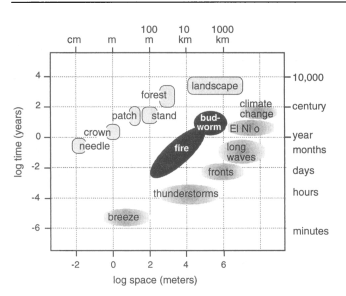
\includegraphics[width=.6\textwidth]{Bilder/Holling-1.png}

    Diagram from (Holling 2001)
  \end{center}
\end{frame}

\begin{frame}{Systemic Structures}
  \begin{center}

    ... of socio-cultural systems ... 
    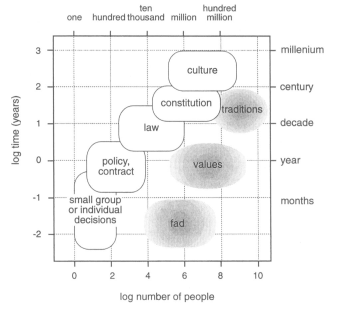
\includegraphics[width=.75\textwidth]{Bilder/Holling-2.png}

    Diagram from (Holling 2001)
  \end{center}
\end{frame}

\begin{frame}{Systemic Structures}

  ... and also of "natural" systems.
  \begin{center}
    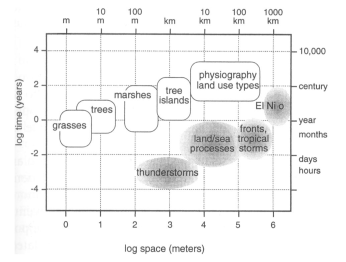
\includegraphics[width=.85\textwidth]{Bilder/Holling-3.png}

    Diagram from (Holling 2001)
  \end{center}
\end{frame}

\begin{frame}{Development of Systemic Structures}

  \emph{Example:} The press department is modernised, industrial robots are
  being used.  How does that affect the other components of the systems?

  What scenarios are conceivable?

\end{frame}

\begin{frame}{Development of Systemic Structures}

  \begin{minipage}{.4\textwidth}
    Which typical scenarios are to be distinguished for systems that develop
    along an attractor?
  \end{minipage}\hfill
  \begin{minipage}{.55\textwidth}\centering
    \begin{tikzpicture}[scale=.55,line width=1pt,transform shape]
      \node (A0) at (0,10) {};
    \node (A4) at (3,8.5) {};
    \node (A1) at (5,7) {};
    \node (A1a) at (7,6.5) {};
    \node (A2) at (0,5) {};
    \node (A3) at (7,0) {};
    \node (A5) at (6.5,4) {};
    \node (A6) at (6,.5) {};
    \draw plot [smooth] coordinates {(A0) (A4) (A1) (A2) (A6) (A3)};
    \node[draw=red] at (4.2,9.2) [rectangle] {$r$ Phase};
    \draw[<->] (2.3,8.1) -- (3.1,7.7) ;
    \node[draw=red] at (6.2,7.5) [rectangle] {$K$ Phase};
    \draw[<->] (4.7,6.5) -- (5.5,6.5) ;
    \node[draw=red] at (8.2,6.5) [rectangle] {$\Omega$ Phase};
    \draw[->] (6.7,5.9) -- (6.6,5.3) ;
    \node[draw=red] at (8,3.8) [rectangle] {$\alpha$ Phase};
    \draw[->] (6.2,3.4) -- (6.1,2.8) ;
    \draw[<->] (5.2,.3) -- (6.2,-.2) ;
    \draw[fill=green] (A4) circle (6pt) ;
    \draw[->,dashed] plot [smooth] coordinates {(A1) (A1a) (A5) (A6)};
    \draw[fill=green] (A1) circle (6pt) ;
    \draw[fill=green] (A1a) circle (6pt) ;
    \draw[fill=green] (A5) circle (6pt) ;
    \draw[fill=green] (A6) circle (6pt) ;
    \node[draw=red,fill=white] at (7.5,0.9) [rectangle] {neue $r$-Phase};
  \end{tikzpicture}
  \end{minipage}
\end{frame}

\begin{frame}{Development of Systemic Structures}
  \begin{center}
    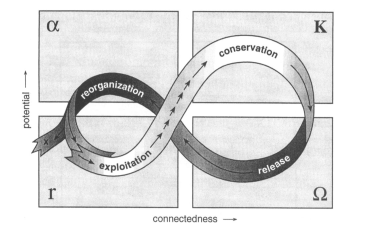
\includegraphics[width=.85\textwidth]{Bilder/Holling-4.png}
  \end{center}
\end{frame}

\begin{frame}{Development of Systemic Structures}
  \begin{center}
    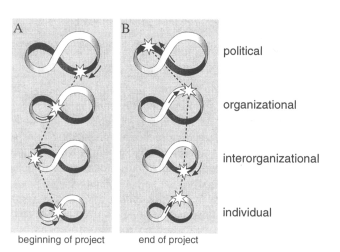
\includegraphics[width=.85\textwidth]{Bilder/Holling-5.png}
  \end{center}
\end{frame}

\end{document}
